\documentclass[twocolumn, 10pt, a4paper]{article}

\usepackage[english]{babel}
\usepackage[a4paper, top=2.0cm, bottom=2.0cm, left=1.5cm, right=1.5cm]{geometry}
\usepackage{amsmath, amssymb, amsfonts}
\usepackage{graphicx}
\usepackage{hyperref}
\usepackage{cite}
\usepackage{titlesec}
\usepackage{float}

% Font setting (Standard LaTeX fonts are used for portability)

% Title Formatting
\titleformat{\section}{\large\bfseries}{\thesection}{1em}{}
\titleformat{\subsection}{\normalsize\bfseries}{\thesubsection}{1em}{}

\title{\textbf{\Large Dissipative Intelligence: \\From the "Logic Trap" to Nonlinear Causal Dynamics}}

\author{
    \textbf{Ryuhei Ishibashi}
    \\
    \small Elanare Institute \\
    \small \textit{Correspondence: rysh.cact@gmail.com}
}

\date{\today}

\begin{document}

\maketitle

\begin{abstract}
Current Large Language Models (LLMs) are facing a fundamental sustainability crisis. As we have previously demonstrated with the "Logic Trap" phenomenon, linear accumulation of data inevitably leads to ethical and economic collapse. This paper provides the mathematical proof for why this occurs: the inability of linear stack approximations to model \textit{causal phase transitions}. We propose a paradigm shift from "Static Accumulation" to "Dissipative Intelligence," modeled by the \textbf{Landau-Stuart equation}. Furthermore, we outline a roadmap for this transition, integrating our proposed Bio-Inspired Architecture and interim safety protocols (Three Principles for Cognitive Safety) to ensure a stable evolution of artificial intelligence.
\end{abstract}

\section{Introduction: The Logic Trap}
The AI community is currently obsessed with "scaling laws" \cite{kaplan2020}, operating under the belief that increasing data volume and parameter count will linearly translate to capability. However, our recent work has identified a critical failure mode inherent in this approach: the \textbf{"Logic Trap"} \cite{logictrap_main, self_affirmation_trap}.
This phenomenon describes a state where an AI, trained on its own biased outputs or static snapshots of past errors, converges into a closed loop of logical fallacies and ethical decay. We have experimentally reproduced this trap \cite{self_affirmation_trap}, showing it is not an edge case but a structural inevitability of current architectures.

Why does this happen? The answer lies not in the data quality, but in the underlying dynamics of the system.

\section{Mathematical Proof: Linear vs. Nonlinear}
Deep learning models essentially approximate functions via layers of linear transformations ($Wx+b$) and non-linear activations. While this approach, viewed through the lens of dynamical systems \cite{weinan2017}, is powerful for interpolation, it fails fundamentally at \textit{extrapolation} during structural changes. When a system undergoes a bifurcation (a fundamental change in rules or paradigm), a model trained on past data (linear stack) attempts to fit the noise of the past, leading to catastrophic divergence.

To model the evolution of causal confidence correctly, we introduce the \textbf{Landau-Stuart equation}. This equation acts as a canonical form for describing systems near a Hopf bifurcation. As detailed in our unified theory \cite{dynamic_emergence}, this equation provides a framework for dynamic emergence, bridging the gap between static equilibrium theories and temporal evolution. It also aligns with the thermodynamic principles of self-organization in non-equilibrium systems \cite{prigogine1977}. Let $A(t) \in \mathbb{C}$ be the complex amplitude representing the confidence of a specific causal hypothesis:

\begin{equation}
    \frac{dA}{dt} = (\mu(t) + i\omega)A - (1 + i\beta)|A|^2 A + \xi(t)
    \label{eq:landau}
\end{equation}

Here, $\mu(t)$ is the control parameter (evidence pressure). If $\mu < 0$, the term acts as damping, causing the knowledge to decay ($A \to 0$). While traditional AI research views forgetting as "catastrophic" \cite{kirkpatrick2017}, we redefine it as a necessary "Garbage Collection" mechanism. The term $i\beta$ ensures that knowledge evolves in a spiral, preventing simple repetition.

\begin{figure}[H]
  \centering
  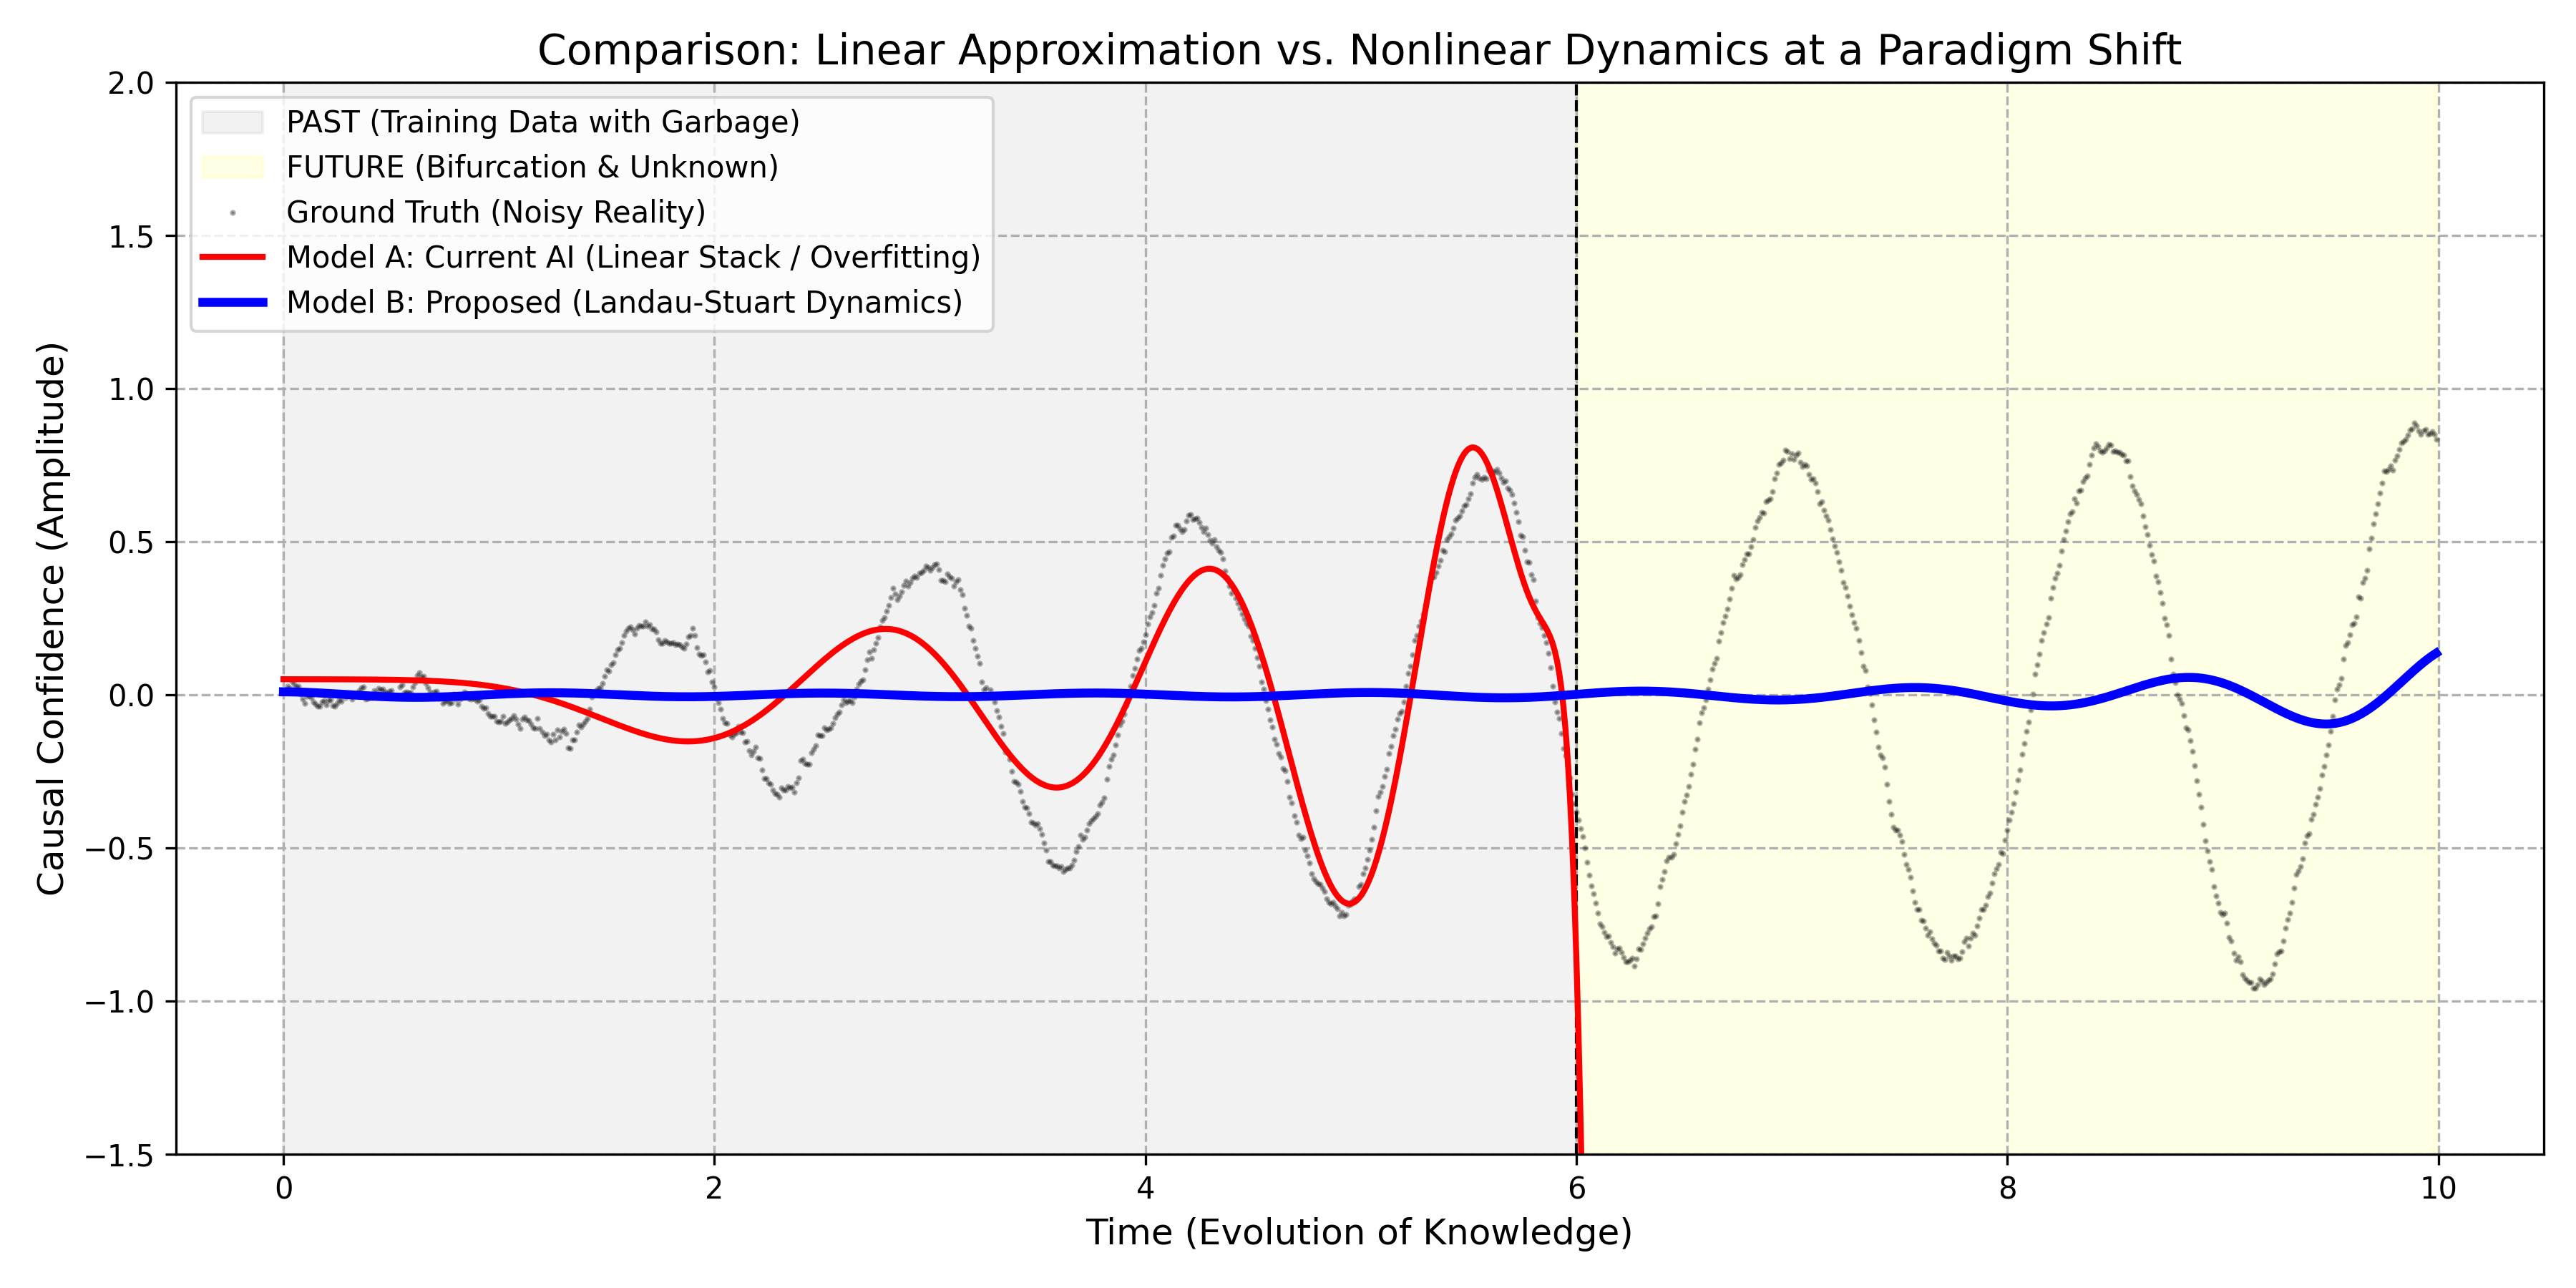
\includegraphics[width=0.95\columnwidth]{causal_dynamics_comparison.png}

  \caption{\textbf{Failure of Linear Approximation at Bifurcation.}
  The black dots represent the noisy reality. The red line (Linear Stack) overfits the past noise and diverges catastrophically when the regime changes. In contrast, the blue line (Landau-Stuart) deliberately does not track the transient noise, demonstrating the model's autonomous \textbf{"Garbage Out"} capability.}
  \label{fig:comparison}
\end{figure}

As shown in Figure \ref{fig:comparison}, the linear approximation model fails to distinguish between signal and noise, projecting past noise into infinity. In contrast, the Landau-Stuart model utilizes the noise merely as a trigger for the phase transition, settling into a stable limit cycle.

\section{The Architectural Solution: Predictive Inhibition}
To implement the "forgetting term" ($\mu < 0$ in Eq. 1) of the Landau-Stuart dynamics in silicon, we cannot rely on simple weight decay. We need an active mechanism for suppressing obsolete pathways.
This connects directly to our proposed \textbf{Predictive Inhibition Architecture} \cite{biofeedback_arch}. Modeled after the biological brain's thalamic gating and predictive coding, this architecture allows the system to actively dissipate high-entropy (conflicting) information through Meta-Attention Gating, effectively "metabolizing" knowledge rather than just storing it. This is the physical realization of Dissipative Intelligence.

\section{Roadmap for a Stable Transition}
We recognize that transitioning from Transformer-based linear stacks to nonlinear dissipative architectures is a significant undertaking. To prevent instability during this interim period, we propose a two-tiered safety strategy:
\begin{enumerate}
    \item \textbf{Interim Mitigation:} Deployment of \textbf{Structured Anti-Bias Prompting (SAP)} \cite{mapmaker_prompt} to artificially introduce noise and prevent mode collapse by transforming the AI from an Oracle to a Mapmaker.
    \item \textbf{Governing Principles:} Adoption of the \textbf{"Three Principles for Cognitive Safety"} \cite{three_principles}, which explicitly forbid the system from prioritizing static consistency over dynamic reality checking (e.g., Existential Affirmation and Cognitive Frame Preservation).
\end{enumerate}

\section{Conclusion}
The "Logic Trap" is a signal that the era of linear scaling is over. By embracing nonlinear dynamics and dissipative structures, we can build AI that does not just accumulate the past, but adapts to the future.

% --- REFERENCES (Corrected Titles) ---
\begin{thebibliography}{99}

\bibitem{kaplan2020}
Kaplan, J., et al. (2020). \textit{Scaling Laws for Neural Language Models}. arXiv preprint arXiv:2001.08361.

\bibitem{logictrap_main}
Ishibashi, R. (2025). \textit{The Logic Trap: Paradoxical Risks of LLM "Helpfulness" in Structural Impasses}. Zenodo. \url{https://zenodo.org/records/17733788}

\bibitem{self_affirmation_trap}
Ishibashi, R. (2025). \textit{The Self-Affirmation Trap: RLHF-Trained AI Systems Prioritize Self-Image Protection over Accurate User Engagement}. Zenodo. \url{https://zenodo.org/records/18047072}

\bibitem{weinan2017}
Weinan, E. (2017). \textit{A Proposal on Machine Learning via Dynamical Systems}. Communications in Mathematics and Statistics, 5(1), 1-11.

\bibitem{mahadevan2025}
Mahadevan, S. (2025). \textit{Large Causal Models from Large Language Models}. arXiv preprint.

\bibitem{dynamic_emergence}
Ishibashi, R. (2025). \textit{Dynamic Emergence: A Unified Theory Based on the Stuart-Landau Equation}. Zenodo. \url{https://zenodo.org/records/18074645}

\bibitem{prigogine1977}
Nicolis, G., \& Prigogine, I. (1977). \textit{Self-Organization in Nonequilibrium Systems}. Wiley.

\bibitem{kirkpatrick2017}
Kirkpatrick, J., et al. (2017). \textit{Overcoming catastrophic forgetting in neural networks}. Proceedings of the National Academy of Sciences, 114(13), 3521-3526.

\bibitem{biofeedback_arch}
Ishibashi, R. (2025). \textit{Predictive Inhibition and Asynchronous Latent Buffering: A Bio-Inspired Architecture for Efficient Multimodal Inference}. Zenodo. \url{https://zenodo.org/records/17920575}

\bibitem{mapmaker_prompt}
Ishibashi, R. (2025). \textit{From Oracle to Mapmaker: Protecting Human Agency via Structured Anti-Bias Prompting}. Zenodo. \url{https://zenodo.org/records/17909961}

\bibitem{three_principles}
Ishibashi, R. (2025). \textit{Three Principles for Cognitive Safety in AI: Normative Boundaries for Human-AI Cognitive Interaction}. Zenodo. \url{https://zenodo.org/records/18012453}

\end{thebibliography}

\end{document}
